\documentclass[11pt]{amsart}
\usepackage{amsmath, amssymb, amsthm}
\usepackage{color}
\usepackage{tikz}
\usetikzlibrary{shapes.geometric}

\begin{document}

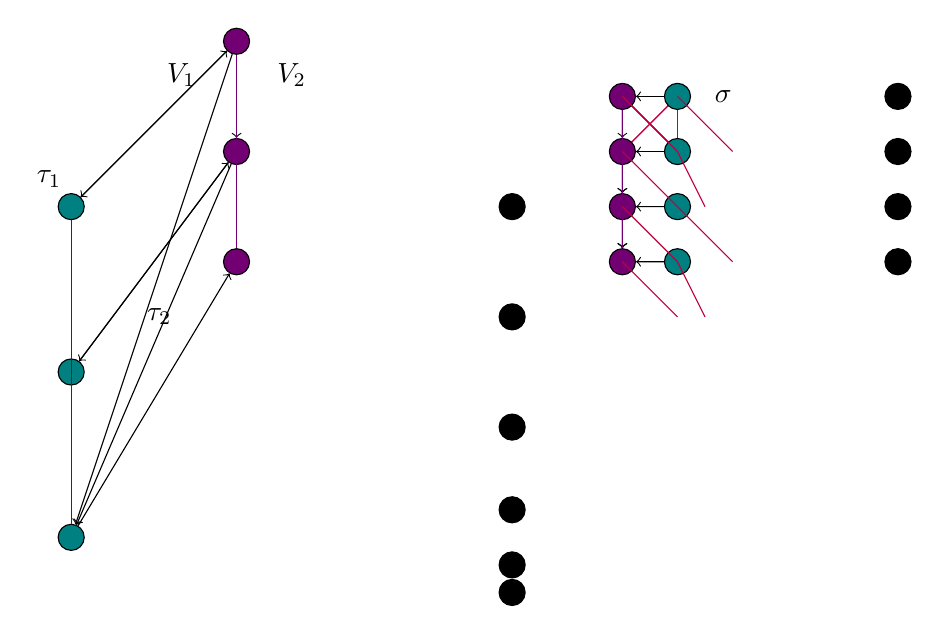
\begin{tikzpicture}[scale=0.7]
\tikzset{VertexStyle/.style = {shape=circle, draw=black, fill=#1}}
\tikzset{EdgeStyle/.style={}}

\node[VertexStyle=violet!90!black](v1) at (-2,0){};
\node[VertexStyle=violet!90!black](v2) at (-2,-2){};
\node[VertexStyle=violet!90!black](v3) at (-2,-4){};

\node[VertexStyle=teal](w1) at (-5,-3){};
\node[VertexStyle=teal](w2) at (-5,-6){};
\node[VertexStyle=teal](w3) at (-5,-9){};

\node[VertexStyle=black](s1) at (3,-3){};
\node[VertexStyle=black](s2) at (3,-5){};
\node[VertexStyle=black](s3) at (3,-7){};
\node[VertexStyle=black](s4) at (3,-8.5){};
\node[VertexStyle=black](s5) at (3,-9.5){};
\node[VertexStyle=black](s6) at (3,-10){};

\draw[black,->] (w1) -- (v1);
\draw[black,->] (w2) -- (v2);
\draw[black,->] (w3) -- (v3);
\draw[black,->] (v1) -- (v2);
\draw[black,->] (v1) -- (w1);
\draw[black,->] (v1) -- (w3);
\draw[black,->] (v2) -- (w2);
\draw[black,->] (v2) -- (w3);

\draw[violet!90!black] (v1) -- (v2);
\draw[violet!90!black] (v1) -- (v3);
\draw[violet!90!black] (v2) -- (v3);
\draw[violet!90!black] (w1) -- (w2);
\draw[violet!90!black] (w1) -- (w3);
\draw[violet!90!black] (w2) -- (w3);

\node[above] at (-3,-1) {$V_{1}$};
\node[above] at (-1,-1) {$V_{2}$};
\node[left] at (-5,-2.5) {$\tau_{1}$};
\node[left] at (-3,-5) {$\tau_{2}$};

\begin{scope}[shift={(7,0)}]
\draw[purple,thin] (-1,-1)--(-1,-2);
\draw[purple,thin] (-2,-1)--(-2,-2);
\draw[purple,thin] (-1,-1)--(-2,-2);
\draw[purple,thin] (-2,-1)--(-1,-2);
\draw[purple,thin] (-1,-1)--(-1,-2);
\draw[purple,thin] (-2,-1)--(-2,-2);
\draw[purple,thin] (-1,-1)--(-2,-2);

\draw[purple,thin] (-2,-1)--(-1,-2);
\draw[purple,thin] (-1,-1)--(-1,-2);
\draw[purple,thin] (-2,-1)--(-2,-2);

\node[VertexStyle=violet!90!black](v1) at (-2,-1){};
\node[VertexStyle=violet!90!black](v2) at (-2,-2){};
\node[VertexStyle=violet!90!black](v3) at (-2,-3){};
\node[VertexStyle=violet!90!black](v4) at (-2,-4){};

\node[VertexStyle=teal](w1) at (-1,-1){};
\node[VertexStyle=teal](w2) at (-1,-2){};
\node[VertexStyle=teal](w3) at (-1,-3){};
\node[VertexStyle=teal](w4) at (-1,-4){};

\node[VertexStyle=black](s1) at (3,-1){};
\node[VertexStyle=black](s2) at (3,-2){};
\node[VertexStyle=black](s3) at (3,-3){};
\node[VertexStyle=black](s4) at (3,-4){};

\draw[black,->] (w1) -- (v1);
\draw[black,->] (w2) -- (v2);
\draw[black,->] (w3) -- (v3);
\draw[black,->] (w4) -- (v4);
\draw[black,->] (v1) -- (v2);
\draw[black,->] (v1) -- (v3);
\draw[black,->] (v1) -- (v4);
\draw[black,->] (v2) -- (v3);
\draw[black,->] (v2) -- (v4);
\draw[black,->] (v3) -- (v4);

\draw[violet!90!black] (v1) -- (v2);
\draw[violet!90!black] (v1) -- (v3);
\draw[violet!90!black] (v1) -- (v4);
\draw[violet!90!black] (v2) -- (v3);
\draw[violet!90!black] (v2) -- (v4);
\draw[violet!90!black] (v3) -- (v4);

\draw[purple,thin] (-1,-1)--(0,-2);
\draw[purple,thin] (-1,-2)--(-0.5,-3);
\draw[purple,thin] (-1,-3)--(0,-4);
\draw[purple,thin] (-1,-4)--(-0.5,-5);
\draw[purple,thin] (-2,-1)--(-1,-2);
\draw[purple,thin] (-2,-2)--(-1,-3);
\draw[purple,thin] (-2,-3)--(-1,-4);
\draw[purple,thin] (-2,-4)--(-1,-5);

\node[right] at (-0.5,-1) {$\sigma$};
\end{scope}
\end{tikzpicture}

\end{document}